\documentclass[12 pt, a4paper]{article}
\usepackage[norsk]{babel}  								% For norsk oppsett
\usepackage[utf8]{inputenc}
\usepackage{amsmath}
\usepackage{amssymb}
\usepackage{graphicx}
\usepackage{subcaption}
\usepackage{hyperref}
\usepackage{fancyhdr}
\usepackage{enumerate}
\usepackage{float}
\usepackage{tikz}
\usepackage{circuitikz}
\usepackage{physics}
\usepackage[includeheadfoot, margin =1cm]{geometry}
%\usepackage{python}
\usepackage[version=3]{mhchem}
\usepackage{siunitx}
\usepackage{todonotes}
\usepackage{xcolor}
\usepackage{lastpage}
\usepackage{listings}
\renewcommand{\exp}[1]{\mathrm{e}^{#1}}

\lstset{basicstyle=\ttfamily,
  showstringspaces=false,
  commentstyle=\color{red},
  keywordstyle=\color{blue}
}

\usepackage[bottom]{footmisc}
\renewcommand\footnoterule{\rule{\linewidth}{0.5pt}}

\setlength{\parindent}{0cm}

\author{Erik Skaar\\ erikfsk@uio.no}





\begin{document}
\pagebreak


\pagestyle{fancy}
\fancyhf{}
\rhead{FYS-MEK1110}
\lhead{Erik Skaar}
\fancyfoot[CE,LO]{Oblig 2}
\fancyfoot[LE,RO]{Page \number\value{page} of \pageref{LastPage}}

\renewcommand{\headrulewidth}{2pt}
\renewcommand{\footrulewidth}{1pt}

% \section{a)}%1

% Konstant kraft gir at $a = F/m$. Posisjonen er da $x(t) = 5/2 t^2$.
% Bytt 5 med 3 eller 1 for Mari og Isak. $v(t) = 3t$ er farten til Mari.
% Python programmet glemte jeg å legge med, håper det går greit.

% \begin{figure}[H]
%     \centering
%     \begin{subfigure}{0.5\textwidth}
%         \centering
%         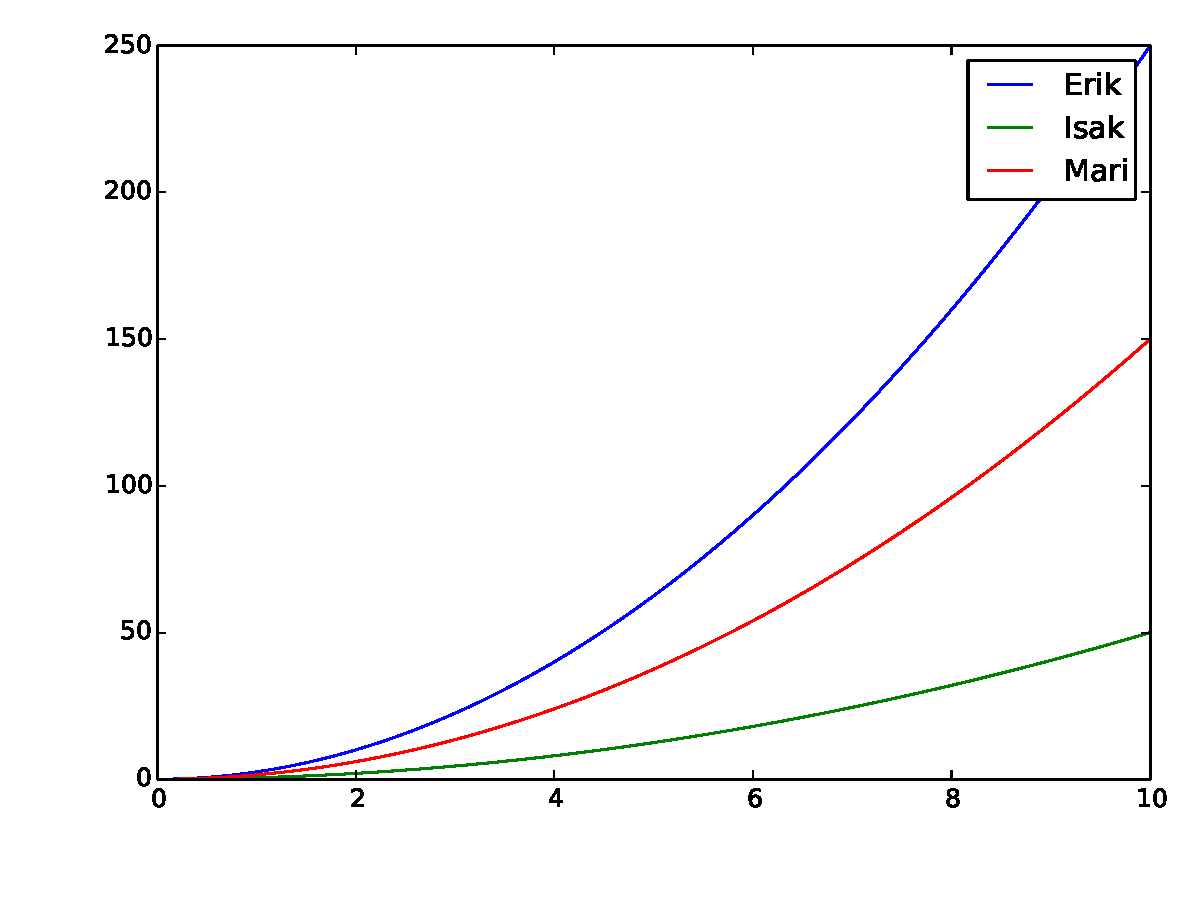
\includegraphics[width=\linewidth]{bilder/standard1.pdf}
%         \caption{}
%     \end{subfigure}%
%     ~
%     \begin{subfigure}{0.5\textwidth}
%         \centering
%         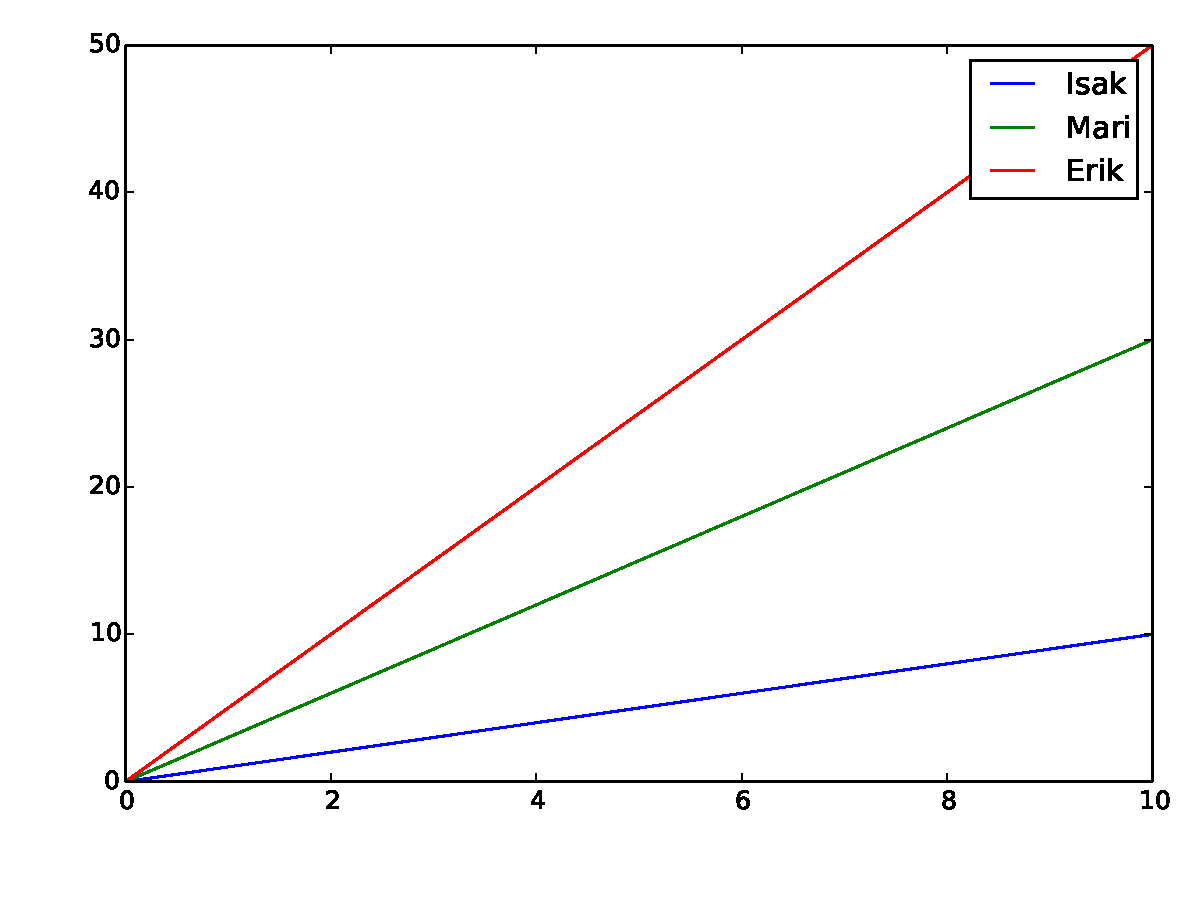
\includegraphics[width=\linewidth]{bilder/standard2.pdf}
%         \caption{}
%     \end{subfigure}
%     \caption{Vis løperene sin hastighet og posisjon}
%     \label{fig:standard}
% \end{figure}

% Erik løper i 50.


% \pagebreak


% \pagebreak



\section*{a)}%1

I denne oppgaven skal vi se på hvordan posisjonen og farten til tre løpere forandrer seg over 10 sekunder. Vi ser borti fra alle andre krefter
enn en konstant drivkraft. Løperene starter i ro og vi setter det som origo.
Siden kraften og massen til løperen er konstant har vi en konstant akselrasjon
i denne oppgaven, $ma = \sum F = F_D \rightarrow a = F_D/m$.
\\
\\
Vi kombinerer dette med at vi vet at:

\begin{align*}
  a(t) &= \frac{\partial ^2x(t)}{\partial  t^2}
  \qquad \rightarrow \qquad
  v(t) =\frac{\partial x(t)}{\partial  t} = \int_{t_0}^{t}a(t) \quad dt
  \qquad \qquad
  x(t) = \int_{t_0}^{t}v(t) \quad dt  = \int_{t_0}^{t}\int_{t_0}^{t}a(t) \quad dt dt
\end{align*}

Dette bruker vi for å finne den generelle formelen for $x(t)$:

\begin{align*}
  x(t)  &= \int_{t_0}^{t}\int_{t_0}^{t}a(t) \quad dt dt
  = \int_{t_0}^{t}\int_{t_0}^{t}a_0 \quad dt dt
  = \int_{t_0}^{t}c_1  + a_0t \quad dt
  =  c_2 + c_1t + \frac{1}{2}a_0t^2
\end{align*}

$c_2$ og $c_1$ er startposisjonen og startfarten respektivt.
Disse vet vi fra introen av oppgaven er null. Setter vi inn for massene og kreftene oppgitt i oppgaven får vi:

\begin{align}
  x(t)_{Isak} = \frac{1}{2}t^2
  \qquad
  x(t)_{Mari} = \frac{3}{2}t^2
  \qquad
  x(t)_{Erik} = \frac{5}{2}t^2
  \label{eq:test_posisjon}
\end{align}

\begin{align}
  v(t)_{Isak} = 1t
  \qquad
  v(t)_{Mari} = 3t
  \qquad
  v(t)_{Erik} = 5t
  \label{eq:test_fart}
\end{align}

\begin{figure}[H]
    \centering
    \begin{subfigure}{0.5\textwidth}
        \centering
        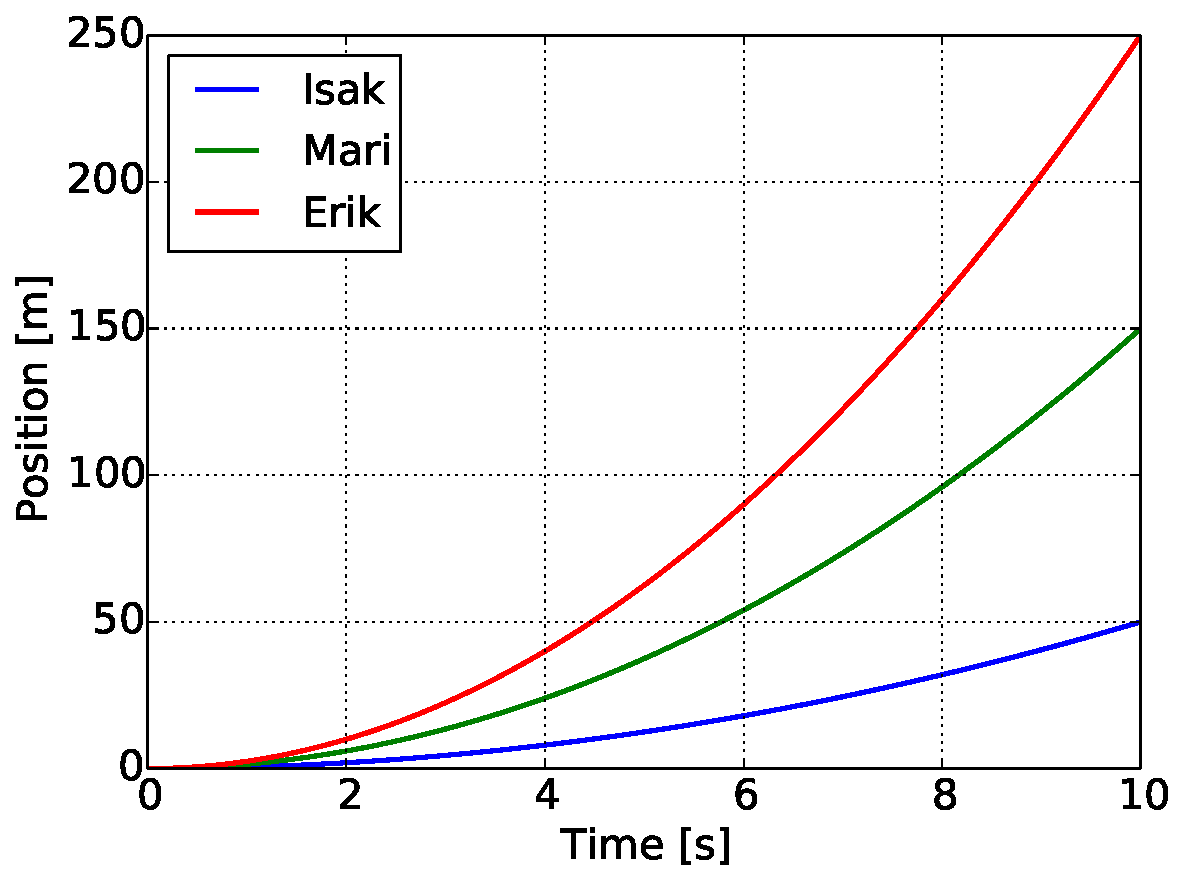
\includegraphics[width=\linewidth]{bilder/advanced1.pdf}
        \caption{}
    \end{subfigure}%
    ~
    \begin{subfigure}{0.5\textwidth}
        \centering
        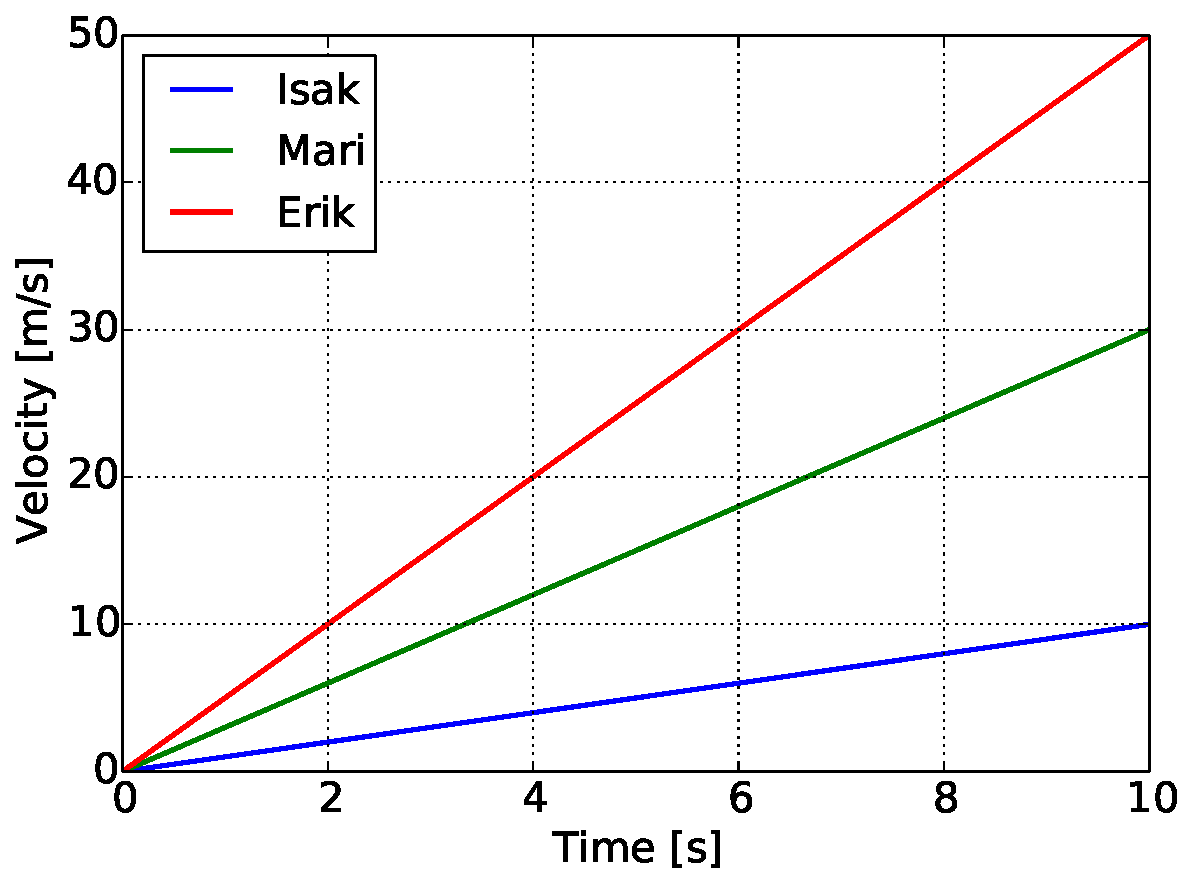
\includegraphics[width=\linewidth]{bilder/advanced2.pdf}
        \caption{}
    \end{subfigure}
    \caption{a) Viser posisjonen til løperene som funksjon av tid.  b) Viser farten til løperene som funksjon av tid. Personene starter i ro og løper med konstant akselrasjon i 10 sekunder.}
    \label{fig:advanced}
\end{figure}

Farten til Erik minner om en bil, Farten til Mari tilhører en gepard og Isak ser
ut som en sneil, men løper etter 10 sek nesten like raskt som Usain Bolt, 12 m/s. For å lage figur
\ref{fig:advanced} implementerte vi formel \ref{eq:test_posisjon} og \ref{eq:test_fart}
i et python script.

\end{document}
